
\begin{frame}{The basic problem}

%\adjincludegraphics[width=0.9\textwidth,trim={0 {.5\height} 0 0 }, clip]{static_figures/survey_and_voting.jpg}

We have a survey population, for whom we observe:
%
\begin{itemize}
 \item Covariates $\x$ (e.g.~race, gender, zip code, age, education level)
 \item Responses $\y$ (e.g.~A binary response to ``do you support Trump'')
\end{itemize}
%

We want the average response in a target population,
in which we observe only covariates.


\splitpage{
    \centering
    \only<1>{
    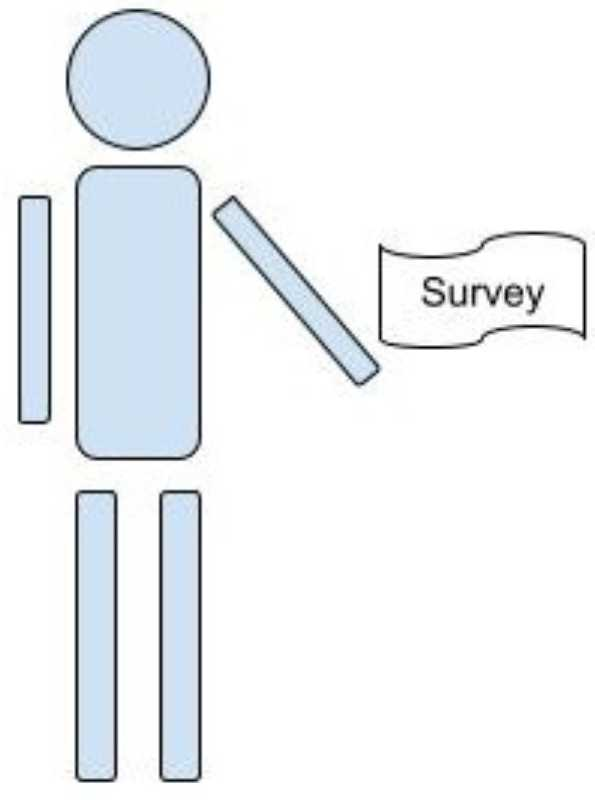
\includegraphics[width=0.5\textwidth]{static_figures/survey_man.jpg}
    }
    \only<2->{
    %
\includegraphics[width=0.5\textwidth]{static_figures/survey_crazy_man.jpg}
    
\includegraphics[width=0.5\textwidth]{static_figures/guinea_pig.png}
    }
}{
    \centering
    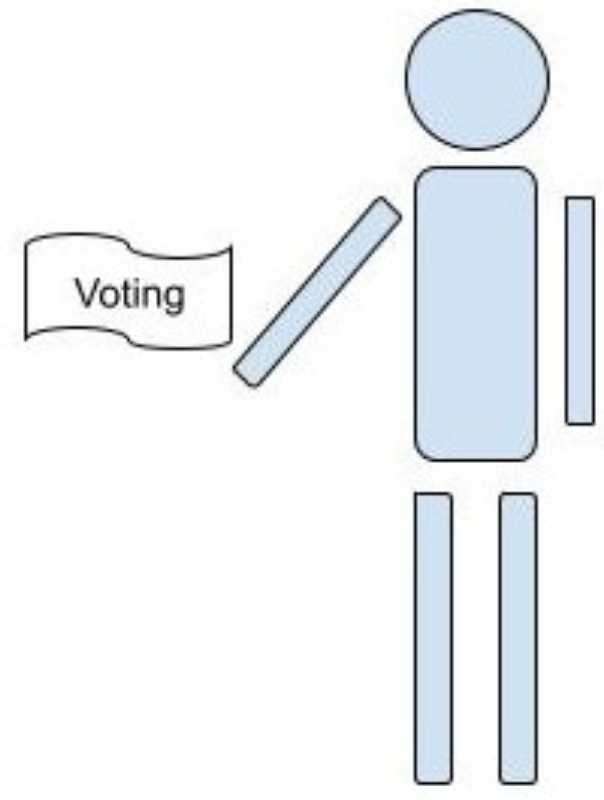
\includegraphics[width=0.5\textwidth]{static_figures/voting_man.jpg}
}

\splitpage{
    \centering
    Observe \surcol{$(\x_i, y_i)$ for $i = 1, \ldots, \nsur$}\\
}{
    \centering
    Observe \tarcol{$\x_j$ for $j = 1, \ldots, \ntar$}\\
}

\onslide<2->{
\textbf{The problem is that the populations may be very different, maybe leading to bias.}
\footnote{Photo copyright: Mark Taylor / \texttt{naturepl.com}}
}

\onslide<3->{
    How can we use the covariates
    to say something about the target responses?
}
%
\end{frame}

%%%%%%%%%%%%%%%%%%%%%%%%%%%%%%%%%%%%%%%%%%%%%%%%%%%%%%%
%%%%%%%%%%%%%%%%%%%%%%%%%%%%%%%%%%%%%%%%%%%%%%%%%%%%%%%
%%%%%%%%%%%%%%%%%%%%%%%%%%%%%%%%%%%%%%%%%%%%%%%%%%%%%%%

\begin{frame}[t]{Two approaches}

We want $\tarcol{\mu := \meantar \y_j}$,
but don't observe target $\tarcol{\y_j}$.  Let $\surcol{\Ysur = \{\y_1, \ldots, \y_{\Nsur}\}}$.

\begin{itemize}
    \item Assume $p(y | \x)$ is the same in both populations,
    \item But the distribution of $\x$ may be different in the survey and target.
\end{itemize}
%
\pause

\splitpagenoline{
    \centering
    \textbf{Calibration weighting}
}{
    \centering
    %\textbf{Multilevel regression and poststratification (MrP)}
    \textbf{Bayesian hierarchical modeling (MrP)}
}
%
%\\\hrulefill\\
\\[1em]
%
\splitpagenoline{
    \centering
    $\blacktriangleright$
    Choose ``calibration weights'' \surcol{$w_i$}\\
    using only the regressors $\x$\\
    (e.g.~raking weights)
}{
    \centering
    $\blacktriangleright$
    Choose $\expect{}{\y \vert \x, \theta} = m(\theta^\trans \x)$,\\
    choose prior $\p(\theta | \Sigma) \p(\Sigma)$\\
    (e.g.~Hierarchical logistic regression)
} \pause
%
\\[1em]
\splitpagenoline{
    \centering
    $\blacktriangleright$ Take
    $\muhatcw = \surcol{\meansur w_i y_i}$
}{
    \centering
    $\blacktriangleright$ Take
    $\tarcol{\yhat_j} =
        \expect{\postsur}{\y | \tarcol{\x_j}}$ and\\
    $\muhatmrp = \tarcol{\meantar \yhat_j}$
}\pause
%
\\[1em]
\splitpagenoline{
    \centering
    $\blacktriangleright$ Dependence %of \surcol{$\muhat_{\cal}$}
    on \surcol{$\y_i$} is clear\\
    % (\surcol{$\w_i$} typically chosen using only $\x$)
}{
    \centering
    $\blacktriangleright$ Dependence %of \surcol{$\muhat_\mrp$}
    on \surcol{$\y_i$} very complicated\\
    (Typically via MCMC draws from $\postsur$)
}\pause
%
\\[1em]
\splitpagenoline{
    \centering
    $\blacktriangleright$ Weights give interpretable diagnostics:
    %
    \begin{itemize}
        \item Frequentist variability
        \item Regressor balance
        \item Partial pooling
        %\item Extrapolation
    \end{itemize}
    %
}{
    \centering
    $\blacktriangleright$ \textbf{Black box}\\
    \pause
    \vspace{1em}
    $\leftarrow$ Today, we'll open the box and provide
        MrP analogues of all these diagnostics
}


\end{frame}


%%%%%%%%%%%%%%%%%%%%%%%%%%%%%%%%%%%%%%%%%%%%%%%%%%%%%%%
%%%%%%%%%%%%%%%%%%%%%%%%%%%%%%%%%%%%%%%%%%%%%%%%%%%%%%%
%%%%%%%%%%%%%%%%%%%%%%%%%%%%%%%%%%%%%%%%%%%%%%%%%%%%%%%

\begin{frame}{Prior work: Equivalent weights for linear models}

\textcite{gelman:2007:struggles} observes that MrP is a weighting estimator when
$\yhat$ is computed with OLS:
$$
\begin{aligned}
% \yhat_j ={}& \x_j^\trans \thetahat  =
%     \x_j^\trans \left(\sumsur \x_i \x_i^\trans \right)^{-1} \sumsur \x_i \y_i \Rightarrow \\
\muhatmrp ={}& \tarcol{\meantar \yhat_j} =
\tarcol{\meantar }
\underbrace{\tarcol{\x_j^\trans} \surcol{\thetahat}}_{\textrm{Linear in }\surcol{\Ysur}}
% =
% \surcol{\sumsur}
% \underbrace{
% \left(\tarcol{\meantar \x_j^\trans}
%     \surcol{
%         \left(\sum_{i'=1}^{\Nsur} \x_{i'} \x_{i'}^\trans \right)^{-1} \x_i
%     }
% \right)
% }_{\surcol{\w^\mrp_i}}  \surcol{\y_i} \\
\end{aligned}
$$

Most existing literature on comparing weighting and MrP focus on such linear models.
\footnote{
    For example,
    \textcite{gelman:2007:struggles,benmichael:2021:multilevel,chattopadhyay:2023:implied}.}

\onslide<2->{
But what if you use a non--linear link function?  Or a hierarchical model?\\
\vspace{2em}
\hrulefill
\begin{displayquote}
``It would also be desirable to use nonlinear methods  ...
but then it would seem difficult to construct
even approximately equivalent weights.  Weighting and fully nonlinear models
would seem to be completely incompatible methods.''
--- \parencite{gelman:2007:strugglesrejoinder}
\end{displayquote}
}
\vspace{1em}

\end{frame}






%%%%%%%%%%%%%%%%%%%%%%%%%%%%%%%%%%%%%%%%%%%%%%%%%%%%%%%
%%%%%%%%%%%%%%%%%%%%%%%%%%%%%%%%%%%%%%%%%%%%%%%%%%%%%%%
%%%%%%%%%%%%%%%%%%%%%%%%%%%%%%%%%%%%%%%%%%%%%%%%%%%%%%%

\begin{frame}[t]{Approximately equivalent weights for (some) logistic regression MrP}

\def\alphav{\mathbf{\alpha}}
%
\begin{itemize}
    \item Suppose the model is $\m(\x^\trans \theta) = \mathrm{Logistic}(\x^\trans \theta)$, with MLE $\thetahat$.
    \item MrP is $\muhatmrp = \tarcol{\meantar \m(\x_j^\trans \thetahat)}$.
\end{itemize}

\pause
The map from $\surcol{\Ysur} \mapsto \m(\x_j^\trans \thetahat)$ is
\emph{inherently nonlinear}.

But \emph{some sample averages}
of $\m(\x_j^\trans \thetahat)$ can be approximately linear.
% \pause
% %
% \begin{block}{Example}
% Suppose
%     $\frac{\tarcol{\ptar}(\x)}{\surcol{\psur}(\x)} \approx \alphav^\trans \x$ for some $\alpha$.
%     \textbf{Then MrP is a \emph{approximately} a CW estimator.}
% \end{block}

\end{frame}



%%%%%%%%%%%%%%%%%%%%%%%%%%%%%%%%%%%%%%%%%%%%%%%%%%%%%%%
%%%%%%%%%%%%%%%%%%%%%%%%%%%%%%%%%%%%%%%%%%%%%%%%%%%%%%%
%%%%%%%%%%%%%%%%%%%%%%%%%%%%%%%%%%%%%%%%%%%%%%%%%%%%%%%

\begin{frame}[t]{Approximately equivalent weights for (some) logistic regression MrP}

\def\alphav{\mathbf{\alpha}}
%
\begin{itemize}
    \item Suppose the model is $\m(\x^\trans \theta) = \mathrm{Logistic}(\x^\trans \theta)$, with MLE $\thetahat$.
    \item MrP is $\muhatmrp = \tarcol{\meantar \m(\x_j^\trans \thetahat)}$.
\end{itemize}

\begin{block}{Example}
Suppose
    $\frac{\tarcol{\ptar}(\x)}{\surcol{\psur}(\x)} \approx \alphav^\trans \x$ for some $\alpha$.
    \textbf{Then MrP is a \emph{approximately} a CW estimator.}
\end{block}
\pause
$$
\vspace{-1em}
\begin{aligned}
\muhatmrp ={}& \tarcol{\meantar \m(\x_j^\trans \thetahat)} \pause
\\ \approx{}&
    \int \tarcol{
        \m(\x^\trans \thetahat) \ptar(\x) d\x
    }
    & \textrm{(Law of large numbers)} \pause
\\ ={}&
    \int
    \surcol{
        \frac{\tarcol{\ptar(\x)}}{\psur(\x)} \m(\x^\trans \thetahat) \psur(\x) d\x
    }
    & \textrm{(Multiply by $\psur(\x) / \psur(\x)$)} \pause
\\ \approx{}&
    \int \surcol{
        \left( \alphav^\trans \x\right) \m(\x^\trans \thetahat) \psur(\x) d\x
    }
    & \textrm{(By assumption)} \pause
\\ \approx{}&
    \surcol{
        \alphav^\trans \meansur \x_i \m(\x_i^\trans \thetahat)
    }
    & \textrm{(Law of large numbers)}\pause
\\={}&
    \surcol{
        \alphav^\trans \meansur \x_i \y_i
    }
    & \textrm{(Property of exponential family MLEs)}
\end{aligned}
$$


\end{frame}


%%%%%%%%%%%%%%%%%%%%%%%%%%%%%%%%%%%%%%%%%%%%%%%%%%%%%%%
%%%%%%%%%%%%%%%%%%%%%%%%%%%%%%%%%%%%%%%%%%%%%%%%%%%%%%%
%%%%%%%%%%%%%%%%%%%%%%%%%%%%%%%%%%%%%%%%%%%%%%%%%%%%%%%

\begin{frame}[t]{Approximately equivalent weights for (some) logistic regression MrP}

\def\alphav{\mathbf{\alpha}}
%
\begin{itemize}
    \item Suppose the model is $\m(\x^\trans \theta) = \mathrm{Logistic}(\x^\trans \theta)$, with MLE $\thetahat$.
    \item MrP is $\muhatmrp = \tarcol{\meantar \m(\x_j^\trans \thetahat)}$.
\end{itemize}
%
\begin{block}{Example}
Suppose
    $\frac{\ptar(\x)}{\psur(\x)} \approx \alphav^\trans \x$ for some $\alpha$.
    \textbf{Then MrP is a \emph{approximately} a CW estimator.}
\end{block}

$$
\begin{aligned}
\muhatmrp =
    \tarcol{\meantar \m(\x_j^\trans \thetahat)} ={}
    \surcol{
        \meansur
        \underbrace{\w_i^\mrp}_{\alphav^\trans \x_i} \y_i
    }  + \textrm{Small error}
\end{aligned}
$$
\only<2>{
But what are the weights?
We don't observe $\frac{\ptar(\x)}{\psur(\x)}$, so can't estimate $\alpha$
directly.
}

\only<3->{
\begin{block}{Key idea (informal)}
\centering
If $\muhatmrp$ is approximately linear, then\footnote{
For MLEs, $\frac{\partial \muhatmrp}{\partial \surcol{\y_i}}$
is given by the implicit function theorem.\footcite{krantz:2012:implicit,giordano:2019:swiss}
}
$\surcol{\w_i^\mrp} \approx \nsur \frac{\partial \muhatmrp}{\partial \surcol{\y_i}}.$
\\[1em]
\end{block}
}

\onslide<4->{
\vspace{0.5em}
\textbf{Note:} The derivatives $\surcol{\w_i^\mrp}$ now have two potentially distinct interpretations:
%
\begin{itemize}
\item \textbf{Equivalent weights: }A characterization of $\Ysur \mapsto \muhatmrp$ for diagnostics
\item \textbf{Implicit weights: }An estimate of $\ptar(\x) / \psur(\x)$
\end{itemize}
%
\vspace{1em}
}

\end{frame}



%%%%%%%%%%%%%%%%%%%%%%%%%%%%%%%%%%%%%%%%%%%%%%%%%%%%%%%
%%%%%%%%%%%%%%%%%%%%%%%%%%%%%%%%%%%%%%%%%%%%%%%%%%%%%%%
%%%%%%%%%%%%%%%%%%%%%%%%%%%%%%%%%%%%%%%%%%%%%%%%%%%%%%%

\begin{frame}[t]{Local weights for nonlinear hierarchical logistic regression MrP}
%
\vspace{-1em}
\begin{itemize}
    \item Suppose the model is $\m(\x^\trans \theta) = \mathrm{Logistic}(\x^\trans \theta)$.
    \item Set a hierarchical prior $\p(\theta \vert \Sigma)\p(\Sigma)$,
            use MCMC to draw from $\post$.
    \item MrP is $\muhatmrp = \tarcol{\meantar \expect{\post}{\m(\x_j^\trans \theta)}}$.
\end{itemize}
%
No reason to think $\Ysur \mapsto \muhatmrp$ is even approximately \textbf{globally} linear.

\onslide<2->{
But can still compute and analyze
$\surcol{\w_i^\mrp} := \nsur \frac{\partial \muhatmrp}{\partial \surcol{\y_i}}$
using Bayesian sensitivity analysis!
\footcite{diaconis:1986:bayesconsistency,gustafson:1996:localposterior,efron:2015:frequentist,giordano:2018:covariances}

\begin{block}{MrP weights for MCMC}
\centering
\vspace{-1em}
$$
\begin{aligned}
\surcol{\w_i^\mrp} :={} \nsur \frac{\partial \muhatmrp}{\partial \surcol{\y_i}}
=
\nsur \tarcol{\meantar}
\underbrace{
    \surcol{
    \cov{\post}{\tarcol{\m(\x_j^\trans \theta)}, \theta^\trans \surcol{\x_i}}
    }
}_{\color{black}\textrm{Can estimate without rerunning MCMC!}}
\end{aligned}
$$
\vspace{-1em}
\end{block}
}

\onslide<3->{

\vspace{0.5em}
The derivatives $\surcol{\w_i^\mrp}$ \emph{again} have two potentially distinct interpretations:
%
\begin{itemize}
\item \textbf{Locally equivalent weights: }A characterization of $\Ysur \mapsto \muhatmrp$ for diagnostics
\item \textbf{Locally implicit weights: }An estimate of $\ptar(\x) / \psur(\x)$
\end{itemize}
%
\onslide<4->{
    \textbf{This talk will focus only on locally equivalent weights.  }(Implicit weights is ongoing work!)
}
%
% \textbf{Note:} The derivatives $\surcol{\w_i^\mrp}$ \emph{again} have two potentially distinct interpretations:
% %
% \begin{itemize}
% %
% \item ``Locally equivalent weights'' \onslide<4->{ $\leftarrow$ \textbf{The present talk will focus on this interpretation}}
% \begin{itemize}
% \item A \emph{local} characterization of $\Ysur \mapsto \muhatmrp$ for diagnostics and interpretation
% \end{itemize}
% \item ``Implicit weights''
% %
% \begin{itemize}
% \item An estimator of $\ptar(\x) / \psur(\x)$ (via Riesz regression applied to the Gateaux derivative)
% \end{itemize}
% \end{itemize}
%
}


\end{frame}




%%%%%%%%%%%%%%%%%%%%%%%%%%%%%%%%%%%%%%%%%%%%%%%%%%%%%%%
%%%%%%%%%%%%%%%%%%%%%%%%%%%%%%%%%%%%%%%%%%%%%%%%%%%%%%%
%%%%%%%%%%%%%%%%%%%%%%%%%%%%%%%%%%%%%%%%%%%%%%%%%%%%%%%

\begin{frame}[t]{Locally equivalent weights for hierarchical logistic regression MrP}
%
\vspace{-1em}
\begin{itemize}
    \item Suppose the model is $\m(\x^\trans \theta) = \mathrm{Logistic}(\x^\trans \theta)$.
    \item Set a hierarchical prior $\p(\theta \vert \Sigma)\p(\Sigma)$,
            use MCMC to draw from $\post$.
    \item MrP is $\muhatmrp = \tarcol{\meantar \expect{\post}{\m(\x_j^\trans \theta)}}$.
\end{itemize}
%
\vspace{2em}
%No reason to think $\Ysur \mapsto \muhatmrp$ is even approximately \textbf{globally} linear.
% \onslide<2->{
    \begin{block}{MrP locally equivalent weights (MrPlew)}
    \centering
    \vspace{1em}
    For new data $\Ytil$, form a \textbf{MrP locally equivalent weighting}:
    $$
    \begin{aligned}
    \muhatmrp[\Ytil] \approx{}& \muhatmrp + \surcol{\sumsur \w_i^\mrp (\ytil_i - \y_i)}
    %\quad\textrm{where}\quad \surcol{\w_i^\mrp} :={} \frac{\partial \muhatmrp}{\partial \surcol{\y_i}}.
    \end{aligned}
    $$
    \vspace{1em}
    \end{block}
    %
% }

\vspace{2em}
% \only<4>{
    \textbf{
        Our task is to rigorously show that even such local weights can be meaningfully
        used diagnostically in the same ways we use global weights.
     }
% }

\end{frame}





%%%%%%%%%%%%%%%%%%%%%%%%%%%%%%%%%%%%%%%%%%%%%%%%%%%%%%%%%%%%%%%%%
%%%%%%%%%%%%%%%%%%%%%%%%%%%%%%%%%%%%%%%%%%%%%%%%%%%%%%%%%%%%%%%%%
%%%%%%%%%%%%%%%%%%%%%%%%%%%%%%%%%%%%%%%%%%%%%%%%%%%%%%%%%%%%%%%%%

\begin{frame}{Real Data: Marital Name Change Survey}
Analysis of changing names after marriage\footnote{
    Based on \textcite{alexander:2019:namechange}.}.

\begin{itemize}
    %
    \item \textbf{Target population:} ACS survey of US population 2017--2022 \footcite{ipumsusa}
    \item \textbf{Survey population:} Marital Name Change Survey (from Twitter)\footnote{
        \textcite{cohen:2019:namechange}
    }
    \item \textbf{Respose:}  Did the female partner keep their name after marriage?
    \item For regressors, use bins of age, education, state, and decade married.
    %
\end{itemize}

\begin{minipage}{0.8\textwidth}
$$
\begin{aligned}
    \textrm{Survey observations:} &&  \surcol{\Nsur} ={}& \AlexNSur  \\
    \textrm{Target observations (rows):} &&  \tarcol{\Ntar} ={}& \AlexNTar \\
    \\
    \textrm{Uncorrected survey mean:} && \surcol{\meansur \y_i} ={}& \AlexSurmean \\
    \textrm{Raking:} && \muhatcw ={}& \AlexRaking \\
    \textrm{MrP:} && \muhatmrp ={}& \AlexMrp
        \quad(\textrm{Post. sd} = \AlexMrpSD)\\
\end{aligned}
$$
\end{minipage}
%
\hfill
%
\begin{minipage}{0.15\textwidth} % Doesn't work with footnotes
\pause

\includegraphics[height=10em]{static_figures/guinea_pig.png}
\end{minipage}
%
\end{frame}


